%\documentclass[aps,prd,nofootinbib]{revtex4-1}
\documentclass[singlepage,notitlepage,nofootinbib,11pt]{revtex4-1}
\usepackage{amsmath}
\usepackage{graphicx}
\usepackage{subfig}
\usepackage{epsfig}
\usepackage{listings}
\usepackage[hidelinks,hyperfootnotes=false,bookmarks=false,colorlinks=true]{hyperref}

\newcommand{\eq}[1]{\begin{align*}#1\end{align*}}
\newcommand{\pmat}[1]{\begin{pmatrix}#1\end{pmatrix}}
\newcommand{\center}[1]{\begin{center}#1\end{center}}
\def\<{\langle}
\def\>{\rangle}
\def\l{\left}
\def\r{\right}


\begin{document}
\title{Problem Set 4 - G6080}
\author{Victor Genty}
\email{vgenty@nevis.columbia.edu}
\homepage{www.nevis.columbia.edu/~vgenty}
\date{\today}
\begin{abstract}
\centering
Source code can be found at \href{https://github.com/vgenty/G6080/tree/master/ps4}{github.com/vgenty/G6080/ps4}
\end{abstract}
\maketitle
\section{Problem 1 - Monte Carlo}
\begin{center}{\it Code for this problem can be found mainly in \verb|ps2/largon/mac/doug_ana.py|, \verb|jackknife.py|, and the monte-carlo implementation in \verb|ps2/largon/src/LArgon.cxx|}\end{center}\\\hspace{1pt}\\
\indent A monte carlo algorithm is implemented in the previous liquid argon code with a few minor adjustments. I created a new method \verb|void LArgon::monte()| which contains the metropolis procedure. The liquid argon code can be switched back and forth between the microcanonical ensemble (constant particle number $N$, volume $V$, and energy $E$) evolved via lennard jones force and the canonical ensemble (constant $N$, $V$, and temperature $T$) evolved via monte carlo. To switch between the two, please edit the line in \verb|develop.cxx| from \verb|b.evolve()| to \verb|b.monte()|. The program output stream will be identical. In the metropolis scheme every ``step'' each particle's position is randomly displaced in a uniform box of side length $\pm 0.1\sigma$ using the function \verb|double LArgon::_get_ran_double(double min, double max)| which returns a random number on the interval min to max. As mentioned in the second problem set the $boost::mt19937$ generator is used. The particle's previous state is stored in $i-1$. The particles are selected in order, given a proposed new position, then the total change in potential energy is is computed. If the total change in potential energy is less, the step is accepted. If the energy is higher, the boltzman weight is computed,
\eq{
  p = e^{-\Delta E/T},
}
for $T$ the fixed energy of the heat bath (a program input parameter). A double precision number $z$ is chosen between 0 and 1. If $z < p$ the move is accepted, if not the particle is placed back in it's initial state. We ran the simulation for $N=864$ particles at a fixed temperature $T=1.069$ with density $\rho=0.75$ for 1000 steps. Only a fraction of the steps are displayed in each graph. The dimensionless energy and pressure are shown in Fig. \ref{energypressure}.
\begin{figure}[h]
  \centering
  \captionsetup[subfigure]{labelformat=empty}
  \subfloat[][]{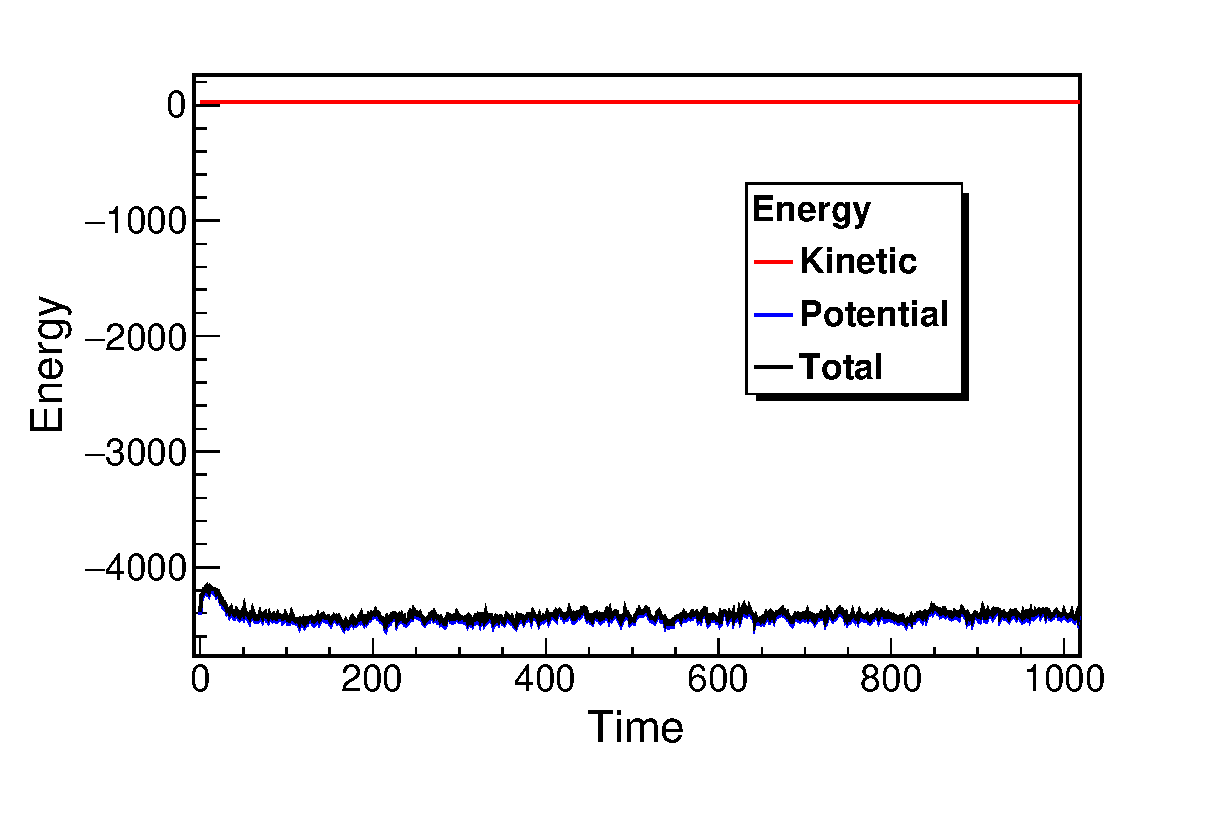
\includegraphics[width=0.5\textwidth]{figures/ener1.eps}}
  \subfloat[][]{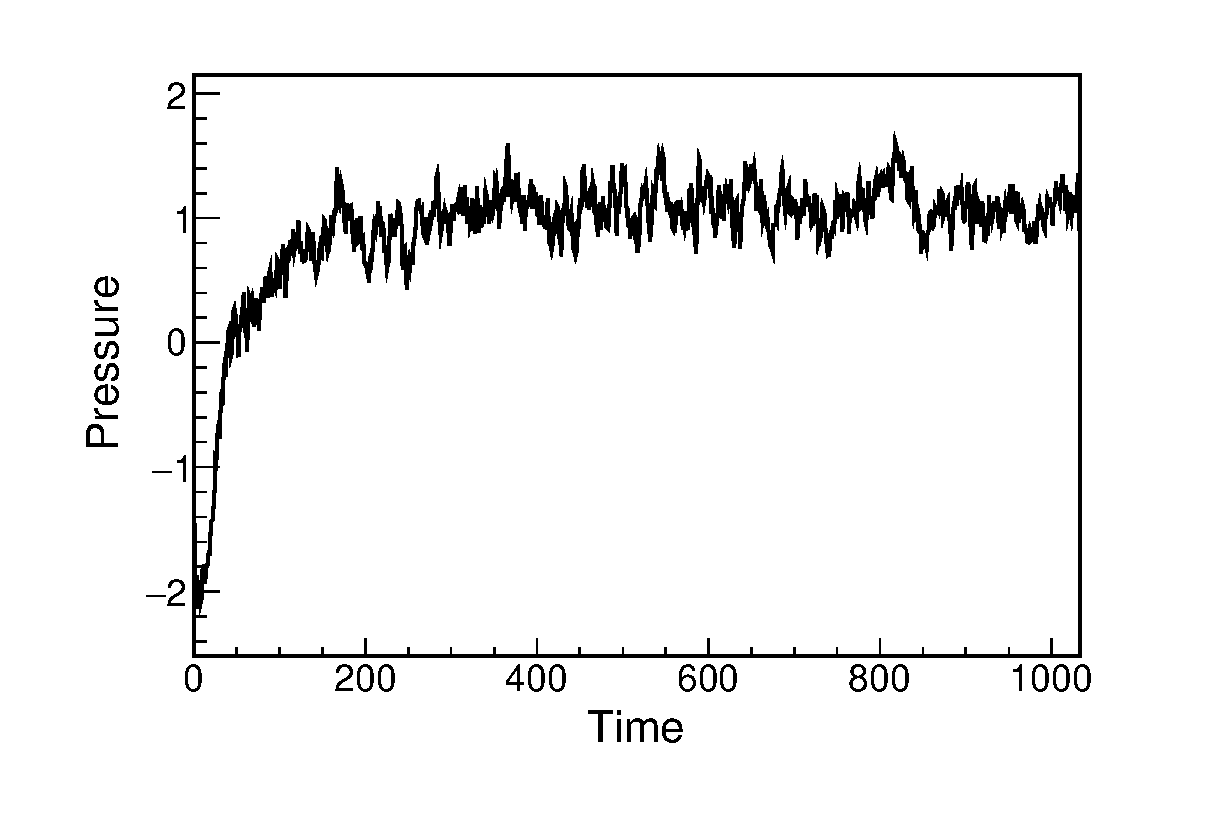
\includegraphics[width=0.5\textwidth]{figures/pres1.eps}}
  \caption{\label{energypressure} Energy and pressure as a function of step. Each step is one full pass of the metroplis algorithm through each particle. The potential energy and pressure thermalize on the order of 100 or so steps.}
\end{figure}
The monte carlo thermalizes roughly on the same order of step size as the velocity-verlet integrator as found in the second problem set. We employ the jackknife to estimate errors on mean value of dimensionless potential energy and pressure (compressability according to the Verlet paper), the results are found in Fig. \ref{jacks}.
\begin{figure}[h]
  \centering
  \captionsetup[subfigure]{labelformat=empty}
  \subfloat[][]{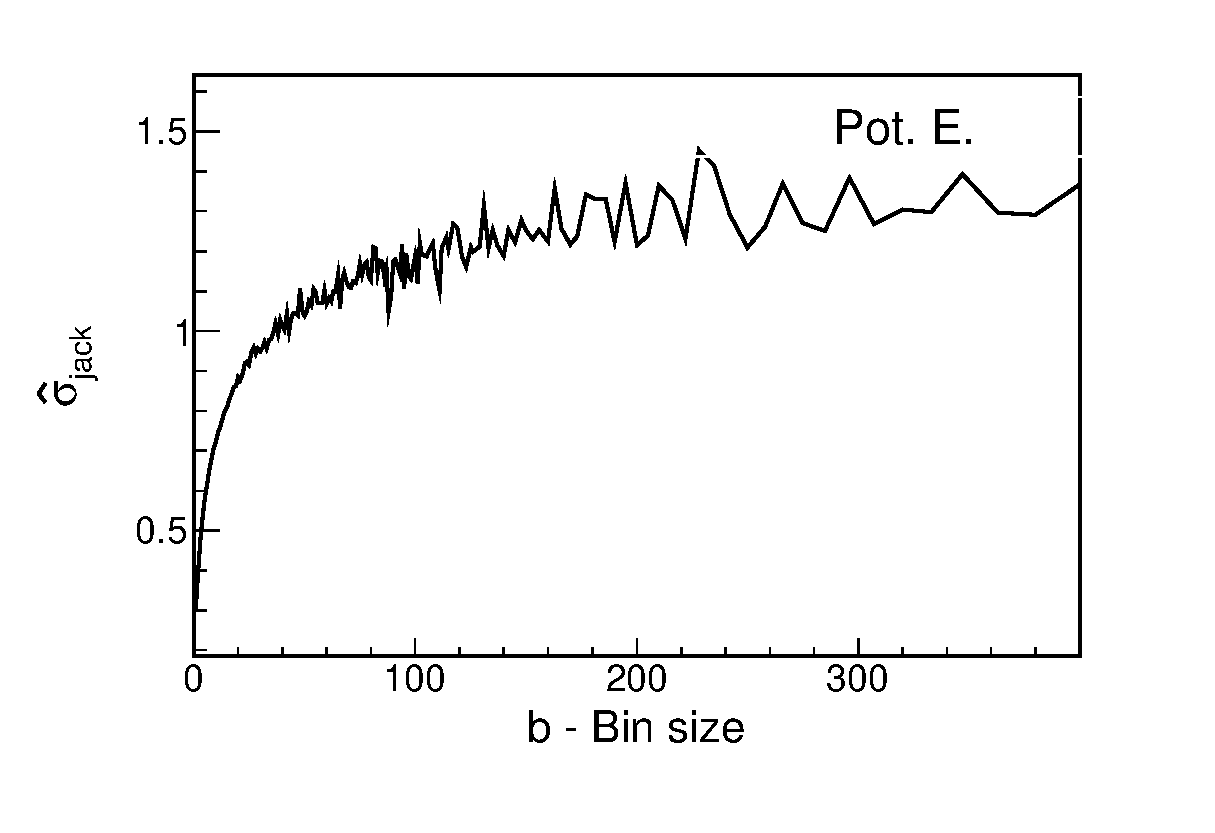
\includegraphics[width=0.5\textwidth]{figures/jack_pote.eps}}
  \subfloat[][]{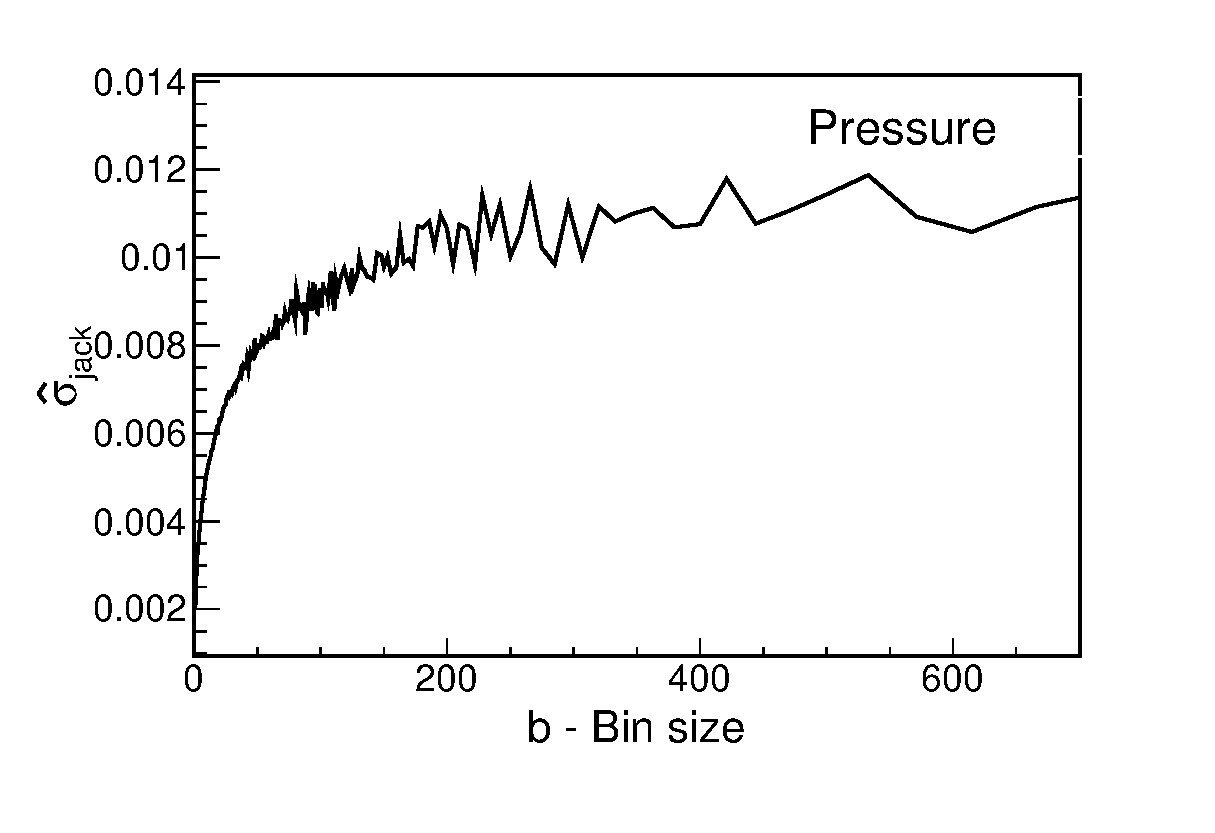
\includegraphics[width=0.5\textwidth]{figures/jack_pressure.eps}}
  \caption{\label{jacks} Jackknife standard deviation for potential energy and pressure. The jackknife method sniffs out the sample standard deviation past the autocorrelation time. We choose a bin size of 300 to accommodate for autocorrelations present in the monte carlo data.}
\end{figure}
We quote a statistical figure and error from the data on the potential energy per particle and the pressure and compare to the Verlet paper. The error on our mean values will be the jackknife standard deviation from a bin size of 300. $U/N$ is the potential energy per particle, and $P$ is the pressure, the results are an average over the final 8000 thermalized data points.
  \begin{center}
    \begin{tabular}{| c | c | c |}\hline
      \hspace{1pt} & $\langle U/N \rangle$ & $\langle P \rangle$ \\ \hline
      Monte Carlo  & -5.1438 $\pm$ 0.0015 &  1.00 $\pm$ 0.01 \\ \hline
      Verlet Paper & -5.19 & 0.90 \\ \hline
    \end{tabular}
  \end{center}
The monte carlo values are fairly close to Verlet's paper The are also consistent with the previous analysis in problem set 2.\\
\indent In the molecular dynamics simulations, the autocorrelation times for observables are related to physics quantities, therefore we study the autocorrelation times for the the potential energy and the virial. Using the standard formula from problem set 3 Fig. \ref{corrs} shows the autocorrelation function for the potential energy and the virial.
\begin{figure}[h]
  \centering
  \captionsetup[subfigure]{labelformat=empty}
  \subfloat[][]{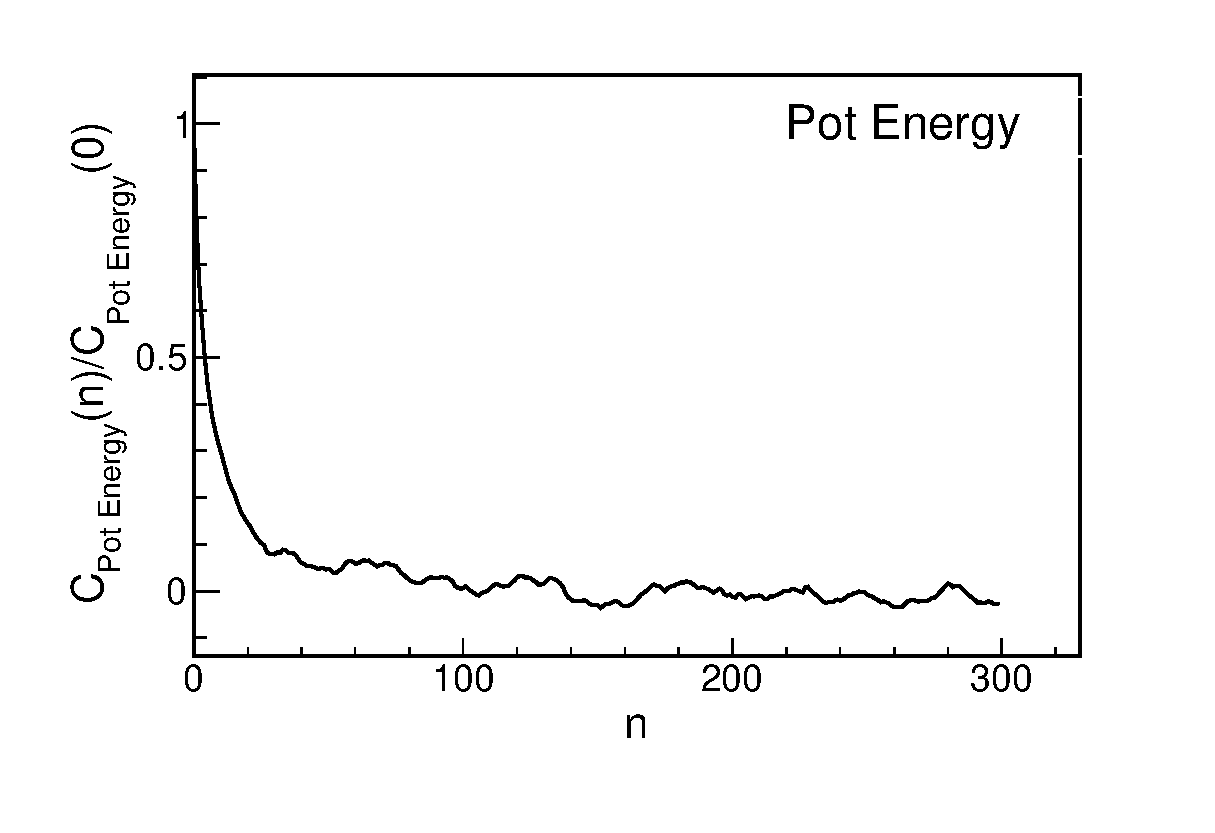
\includegraphics[width=0.5\textwidth]{figures/pot_energy.eps}}
  \subfloat[][]{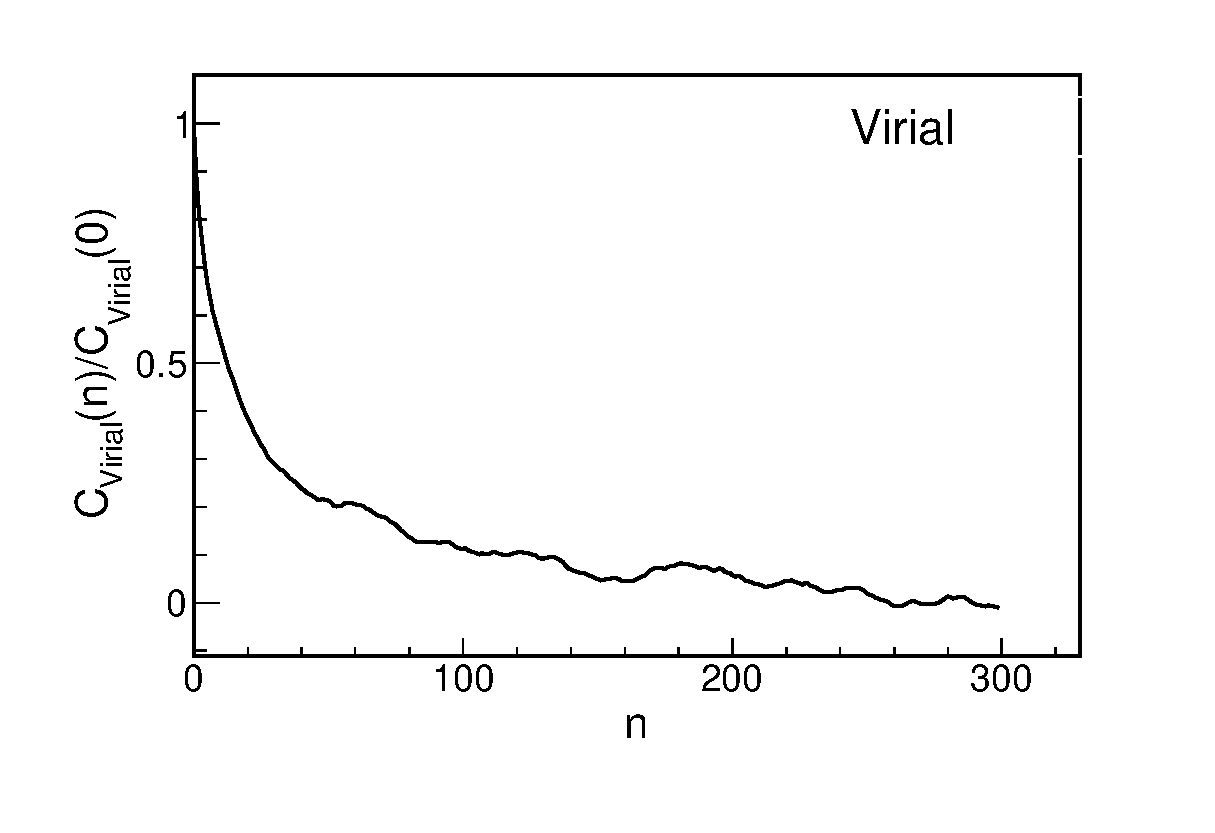
\includegraphics[width=0.5\textwidth]{figures/virial.eps}}
  \caption{\label{corrs} Normalized autocorrelation functions for the potential energy and the virial calculation. The autocorrelations disappear after roughly 300 values during thermalization.}
\end{figure}
The integrated autocorrelations times can be found in the following table with a value of $n_{\text{cut}} = 300$.
  \begin{center}
    \begin{tabular}{| c | c |}\hline
      $\tau_{\text{potential}}$ & $\tau_{\text{pressure}}$ \\ \hline
        10.907 & 38.004\\ \hline
    \end{tabular}
  \end{center}
\clearpage
\section{Problem 2 - Wolff Ising with Metropolis}
I modified \verb|custer.C| to include presence on non-zero magnetic field. Each step, a cluster is identified by Wolff recursion and stored in \verb|int cluster[N*N]|. The total cluster magnetization $M_c$ is computed. If $B\cdot M_c <= 0$ the cluster is flipped 100\% of the time as is it energetically favorable. If positive, the boltzman weight is computed and a random number chosen. If the random number is less than the boltzman weight the spin is flipped in the direction of the field. The weaker the magnetic field the more likely spins of opposite orientation are flipped. The spin state is outputted into a data file \verb|the_spins.dat| as well as the absolute magnetization as a function of step. The program has also been modified to access three input prameters: temperature, magnetic field, and number of steps. The number of spins is hard coded. 

\end{document}
